\chapter{Results }
The expected output of the sign language detection system involves the accurate and real-time recognition of specific sign language gestures, such as "Hello," "No," "I Love You," and other predefined labels. Here's a detailed description of the expected outcomes:

Real-Time Gesture Recognition:
The system should be able to process video input from a camera and recognize the sign language gestures in real-time. When a user performs a gesture, the system should quickly and accurately identify the gesture and display the corresponding label.

Accuracy and Reliability:
The system is expected to achieve high accuracy in recognizing gestures. For instance, when the user signs "Hello," the system should correctly label the gesture as "Hello" with minimal errors. Similar accuracy is expected for other gestures such as "No," "I Love You," "Yes," "Thank You," and "OK."

Visual Feedback:
The system should provide visual feedback by displaying the recognized gesture label on the screen. This feedback helps the user confirm that the gesture was correctly recognized. Additionally, the system may highlight the detected hand landmarks or gestures on the video feed to enhance user interaction.

Text and Spoken Translations:
In addition to visual feedback, the system can provide textual and spoken translations of the recognized gestures. For example, when the user signs "I Love You," the system will display the text "I Love You" on the screen and optionally convert it to spoken words using text-to-speech technology.

Multi-Gesture Recognition:
The system should be capable of recognizing a variety of gestures beyond "Hello," "No," and "I Love You." It should accurately identify other labels such as "Yes," "Thank You," and "OK," making it versatile for different communication needs.
\newpage

\section{Output}
\subsection{I LOVE YOU}
\begin{figure}[ht]
    \centering
    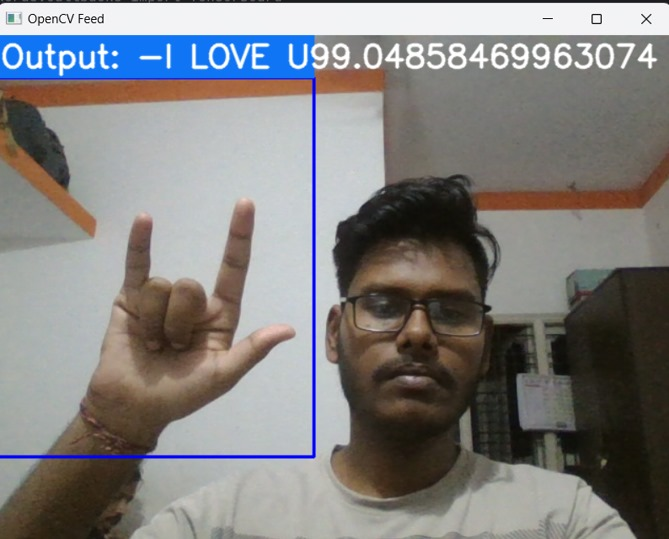
\includegraphics[width=1.0\linewidth]{images/love.jpg}
    \caption{This figure show the I LOVE YOU sign detection}
    \label{fig:flowchart-sign-language}
\end{figure}
\newpage
\subsection{OKAY}
\begin{figure}[ht]
    \centering
    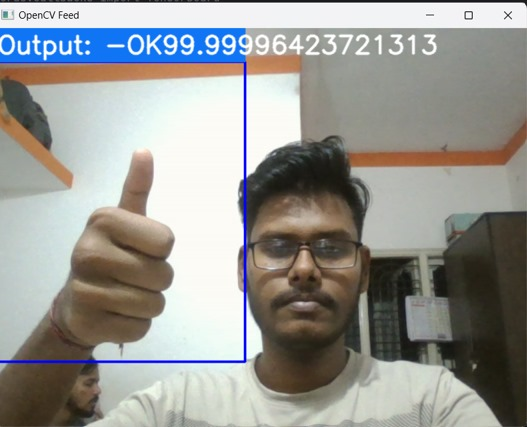
\includegraphics[width=1.0\linewidth]{images/okay.jpg}
    \caption{This figure show the OKAY sign detection}
    \label{fig:flowchart-sign-language}
\end{figure}
\newpage
\subsection{NO}
\begin{figure}[ht]
    \centering
    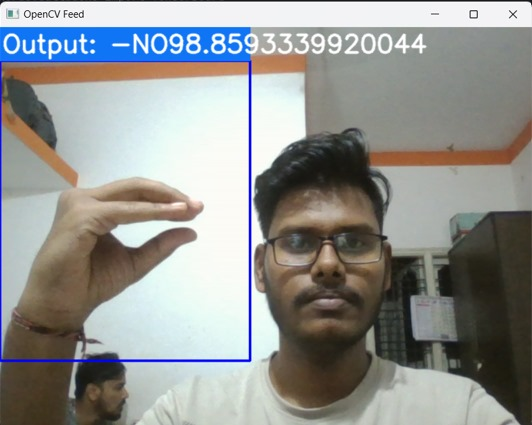
\includegraphics[width=1.0\linewidth]{images/no.jpg}
    \caption{This figure show the NO sign detection}
    \label{fig:flowchart-sign-language}
\end{figure} 
\newpage
\subsection{THANK YOU}
\begin{figure}[ht]
    \centering
    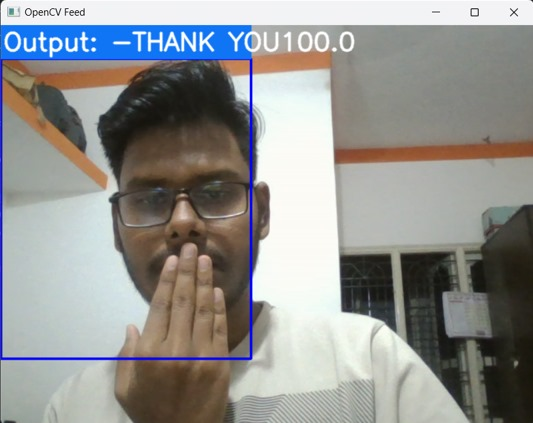
\includegraphics[width=1.0\linewidth]{images/thank you.jpg}
    \caption{This figure show the THANK YOU sign detection}
    \label{fig:flowchart-sign-language}
\end{figure} 

\newpage
\section{Advantages}

\begin{itemize}
    \item Enhanced Accessibility:
   - The primary advantage of a sign language detection system is its potential to enhance communication for the deaf and hard-of-hearing community. By translating sign language into spoken or written text in real-time, it bridges the communication gap between sign language users and those who do not understand it.

    \item Real-Time Translation:
   The use of Recurrent Neural Networks (RNNs) and Long Short-Term Memory (LSTM) networks allows for the processing and recognition of sign language gestures in real-time. This immediate translation capability is crucial for facilitating natural and seamless conversations.

    \item  Cultural Inclusivity:
   Implementing such a system promotes cultural inclusivity by acknowledging and supporting the use of sign language. It can help raise awareness and encourage the integration of sign language into various public and private sectors.


    \item Learning and Education:
   The system can serve as an educational tool, aiding in the teaching and learning of sign language. It can be used in classrooms or self-study applications, providing instant feedback to learners.
   \item Versatility and Scalability:
   The technology can be adapted to recognize multiple sign languages and dialects, making it versatile for global applications. Additionally, as the system is based on machine learning, it can continuously improve and scale with more data and advanced algorithms.

   \item Cost-Effective Solution:
   Compared to hiring human interpreters, an automated sign language detection system can provide a more cost-effective and readily available solution for institutions and individuals needing translation services.

    \end{itemize}
    
\section{Applications}

\begin{itemize}
    \item Healthcare:
   In healthcare settings, the system can facilitate communication between medical professionals and deaf or hard-of-hearing patients, ensuring that medical advice and instructions are accurately conveyed.


    \item Education:
   Schools and universities can use the system to support deaf students, providing real-time translation of lectures and interactive participation in class discussions.


    \item  Customer Service:
   Businesses can implement the system in customer service environments, such as banks, retail stores, and service centers, to assist customers who use sign language, thereby improving customer satisfaction and inclusivity.



    \itemPublic Services:
   Government offices and public service providers can integrate the system to ensure that their services are accessible to all citizens, including those who communicate through sign language.

   \item Media and Entertainment:
   The system can be used in media, such as TV shows, news broadcasts, and online content, to provide real-time sign language interpretation, making content accessible to a broader audience.


   \item Workplace Communication:
   In professional environments, the system can enhance workplace inclusivity by enabling effective communication between deaf employees and their colleagues, fostering a more inclusive and productive work environment.

   \item Social Interactions:
   On a personal level, the system can be used in everyday social interactions, helping deaf individuals communicate more easily with friends, family, and the wider community.



    \end{itemize}

